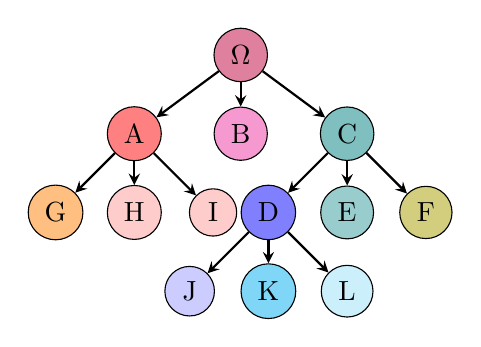
\begin{tikzpicture}[]
    \tikzstyle{space} = [circle, minimum width=0.6cm,text centered, draw=black]
    \tikzstyle{arrow} = [thick,->,>=stealth]

      \node(space)[space, fill = purple!50]{$\Omega$};


 
        %depth 1
        \node(B)[space, fill = magenta!40, below of = space, yshift = -0cm]{B};
        \node(A)[space, fill = red!50, left of = B, xshift = -10pt]{A};
        \node(C)[space, fill = teal!50,  right of = B, xshift = 10pt]{C};
        \draw[arrow] (space) -- (A);
        \draw[arrow] (space) -- (B);
        \draw[arrow] (space) -- (C);
    
    \onslide<2->{ % First loop
    %depth 1
    \node(E)[space, fill = teal!40, below of = C, yshift = -0cm]{E};
    \node(D)[space, fill = blue!50, left of = E]{D};
    \node(F)[space, fill = olive!40,  right of = E]{F};
    \draw[arrow] (C) -- (E);
    \draw[arrow] (C) -- (D);
    \draw[arrow] (C) -- (F);
    }

    \onslide<3->{
    %depth 2
    \node(H)[space, fill = red!20, below of = A]{H};
    \node(G)[space, fill = orange!50, left of = H]{G};
    \node(I)[space, fill = pink!80,  right of = H]{I};
    \draw[arrow] (A) -- (G);
    \draw[arrow] (A) -- (H);
    \draw[arrow] (A) -- (I);

    \node(K)[space, fill = cyan!50, below of = D]{K};
    \node(J)[space, fill = blue!20, left of = K]{J};
    \node(L)[space, fill = cyan!20,  right of = K]{L};
    \draw[arrow] (D) -- (J);
    \draw[arrow] (D) -- (K);
    \draw[arrow] (D) -- (L);
    }
    
    

\end{tikzpicture}